\chapter{Classification}

% ---------- Confusion Matrix ----------
\thispagestyle{customstyle}
\section{Confusion Matrix}
\subsection{Confusion Matrix}

% ---------- FPR ----------
\clearpage
\section{FPR}
\subsection{False Positive Rate}
\thispagestyle{classificationstyle}

The False Positive Rate (FPR), also known as the false alarm ratio or fall-out, measures how often negative instances are incorrectly classified as positive in binary classification.

\begin{center}
\tikz{
\node[inner sep=2pt, font=\Large] (a) {
{
$\displaystyle
FPR = \frac{{\color{cyan}FP}}{{\color{cyan}FP} + {{\color{nmlpurple}TN}}}
$
}
};
\draw[-latex,cyan, semithick] ($(a.north)+(1.3,0.05)$) to[bend left=15] node[pos=1, right] {False positives} +(1,.5); 
% \draw[-latex,teal!70!green, semithick] ($(a.south)+(2.1,0.1)$) to[bend right=15] node[pos=1, right] {Mean of targets} +(1,-.5); 
\draw[-latex,nmlpurple, semithick] ($(a.south)+(1.5,-0.05)$) to[bend left=15] node[pos=1, left] {True negatives} +(-1,-.5); 
}
\end{center}

FPR ranges from 0 (no false alarms) to 1 (all predicted positives are incorrect). FPR can also be interpreted as the probability that a negative instance will be incorrectly identified as positive.

\textbf{When to use FPR?}

Use FPR when you need to evaluate how well a classifier avoids false positives, especially when false positives have significant costs, like in medical diagnostics or security systems. It's also useful for understanding the trade-off between true positive rate (sensitivity) and false positive rate.

\coloredboxes{
\item It provides a clear and intuitive measure of a classifier's false positive performance.
\item It helps identify scenarios where the classifier is overly sensitive and prone to false alarms.
}
{
\item FPR does not consider true positive instances.
\item FPR can be sensitive to class imbalance, as it may be easier to achieve a low FPR when the negative class is dominant.
\item FPR doesn't exist in isolation; it's often important to show its relationship with another key metric. (e.g., TPR, Precision, Recall).
}


\clearpage
\thispagestyle{customstyle2}


\begin{figure*}[ht!]
    \centering
    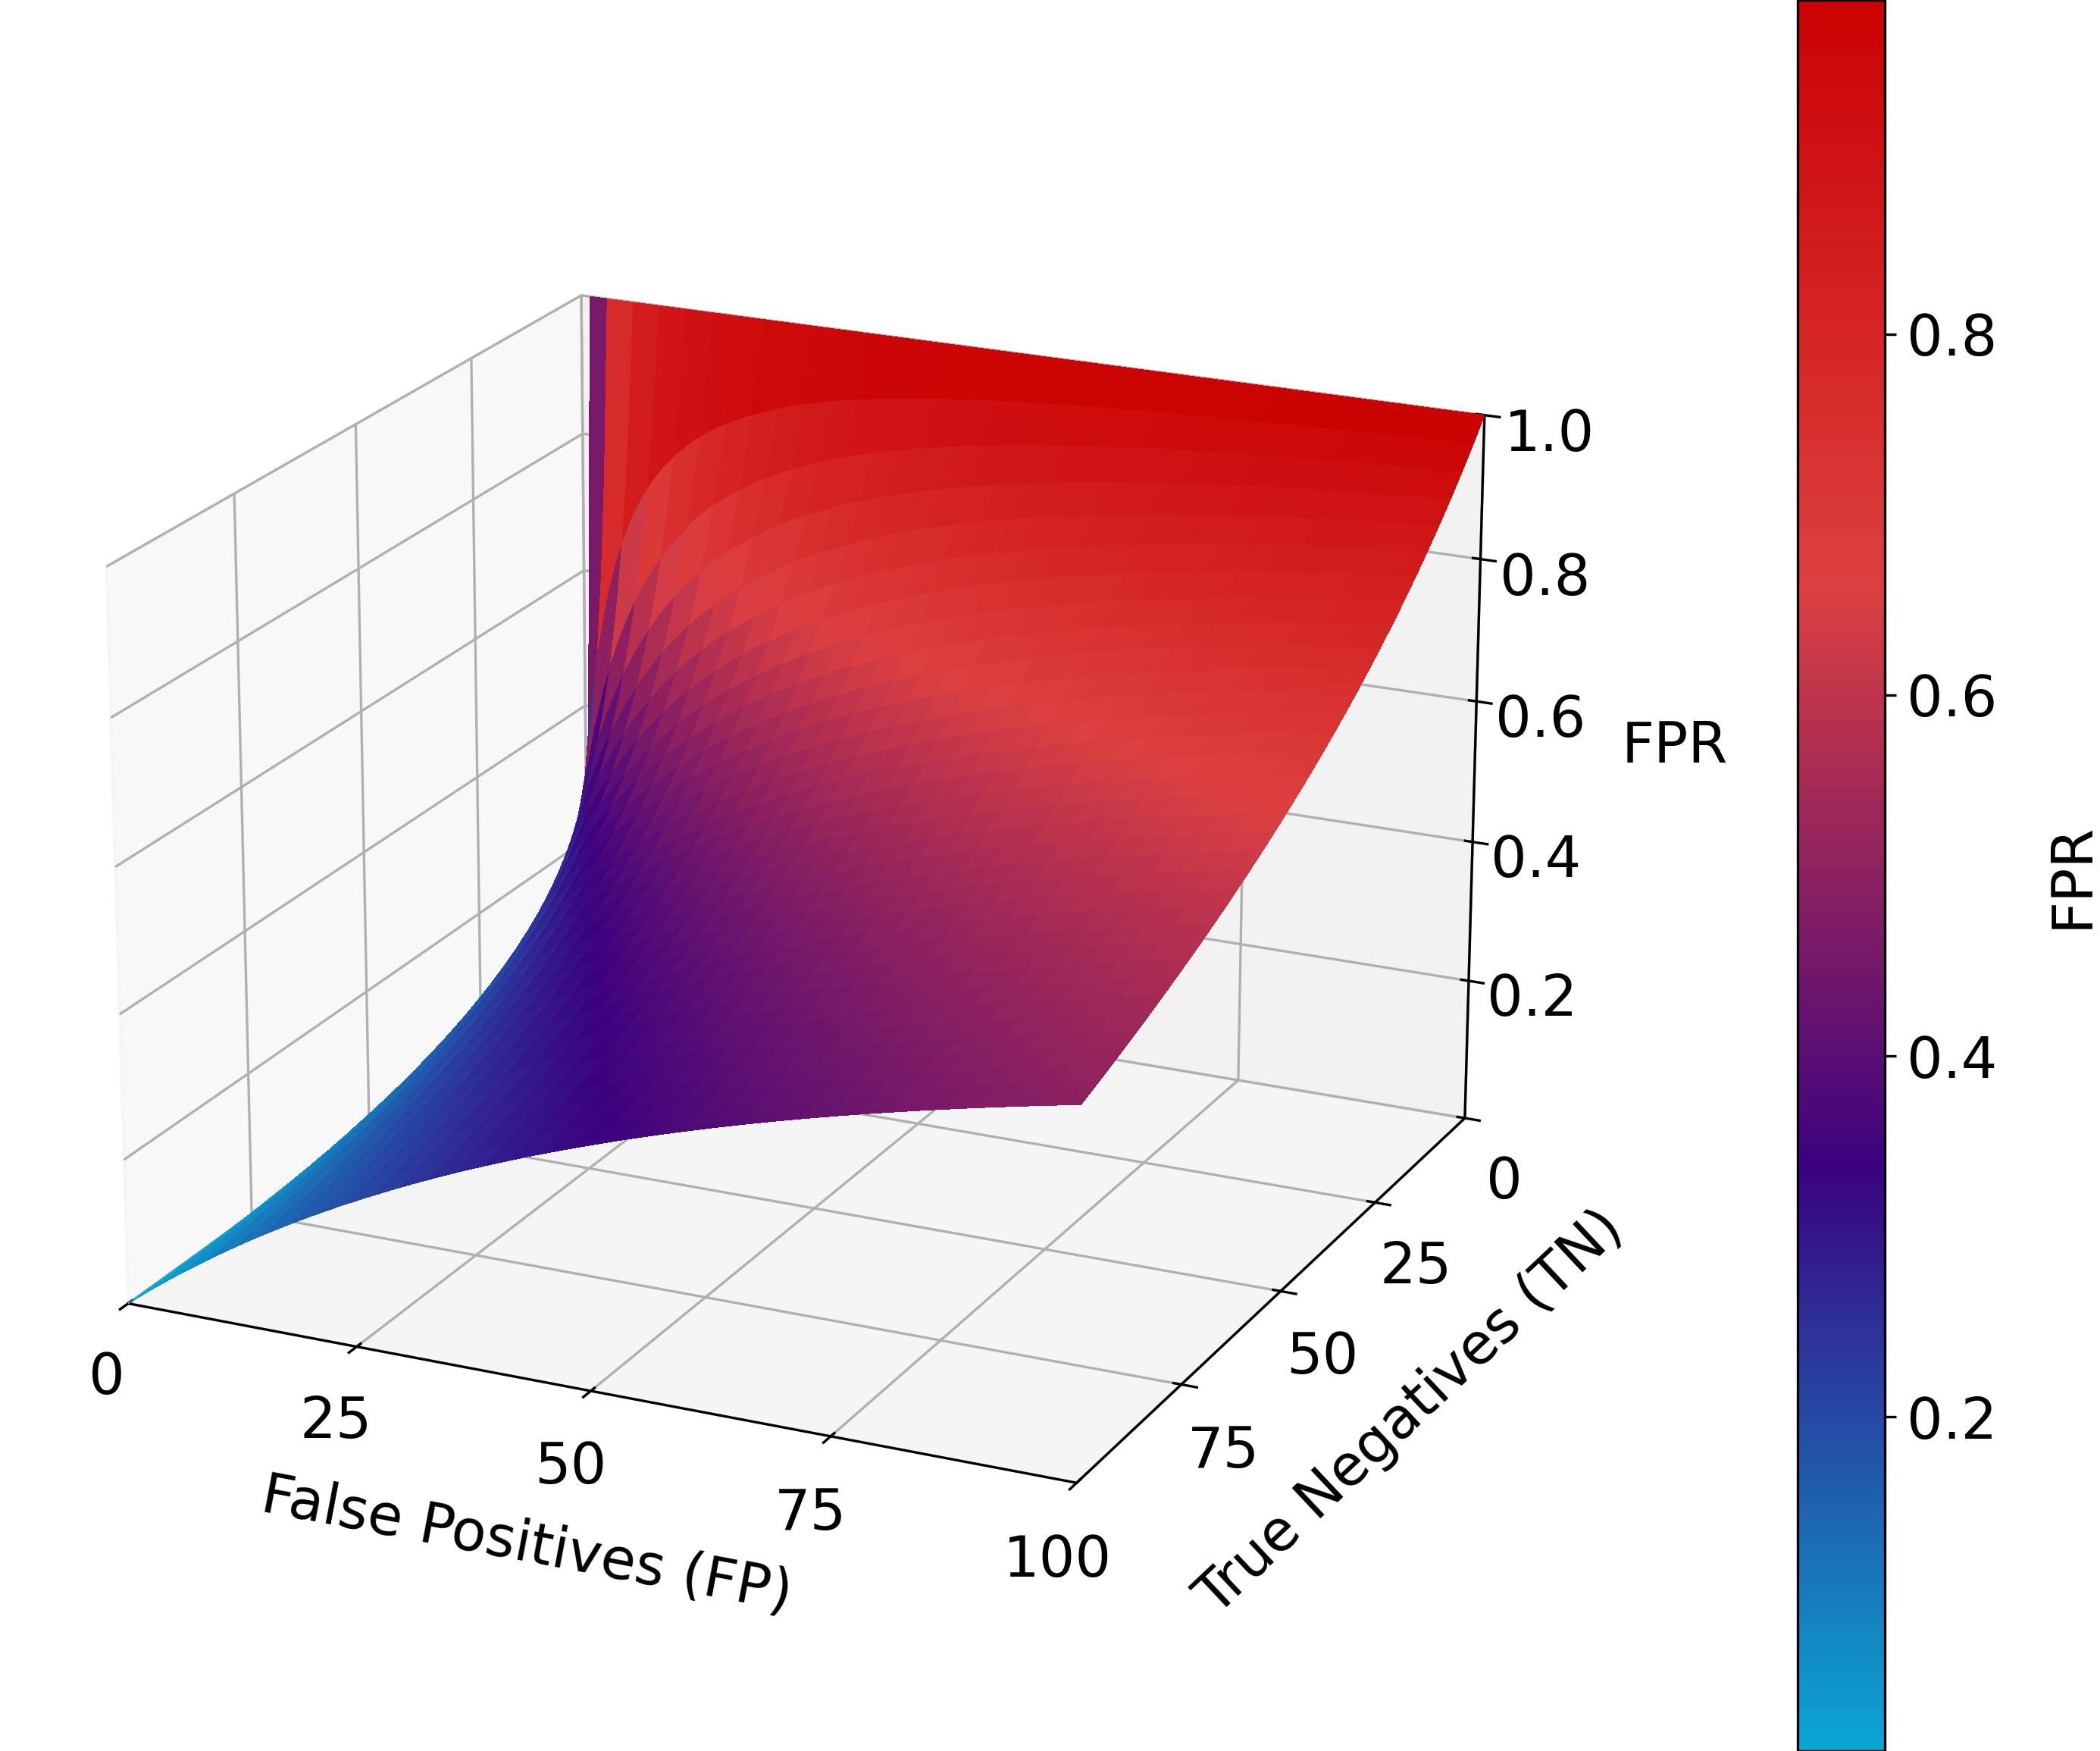
\includegraphics[width=0.7\textwidth]{figures/FPR_3d_surface.png}
    % \caption{Caption}
    \label{fig1}
\end{figure*}

\begin{wrapfigure}{r}{0.55\textwidth}
    \centering
    \vspace{-20pt} % Adjust vertical alignment if needed
    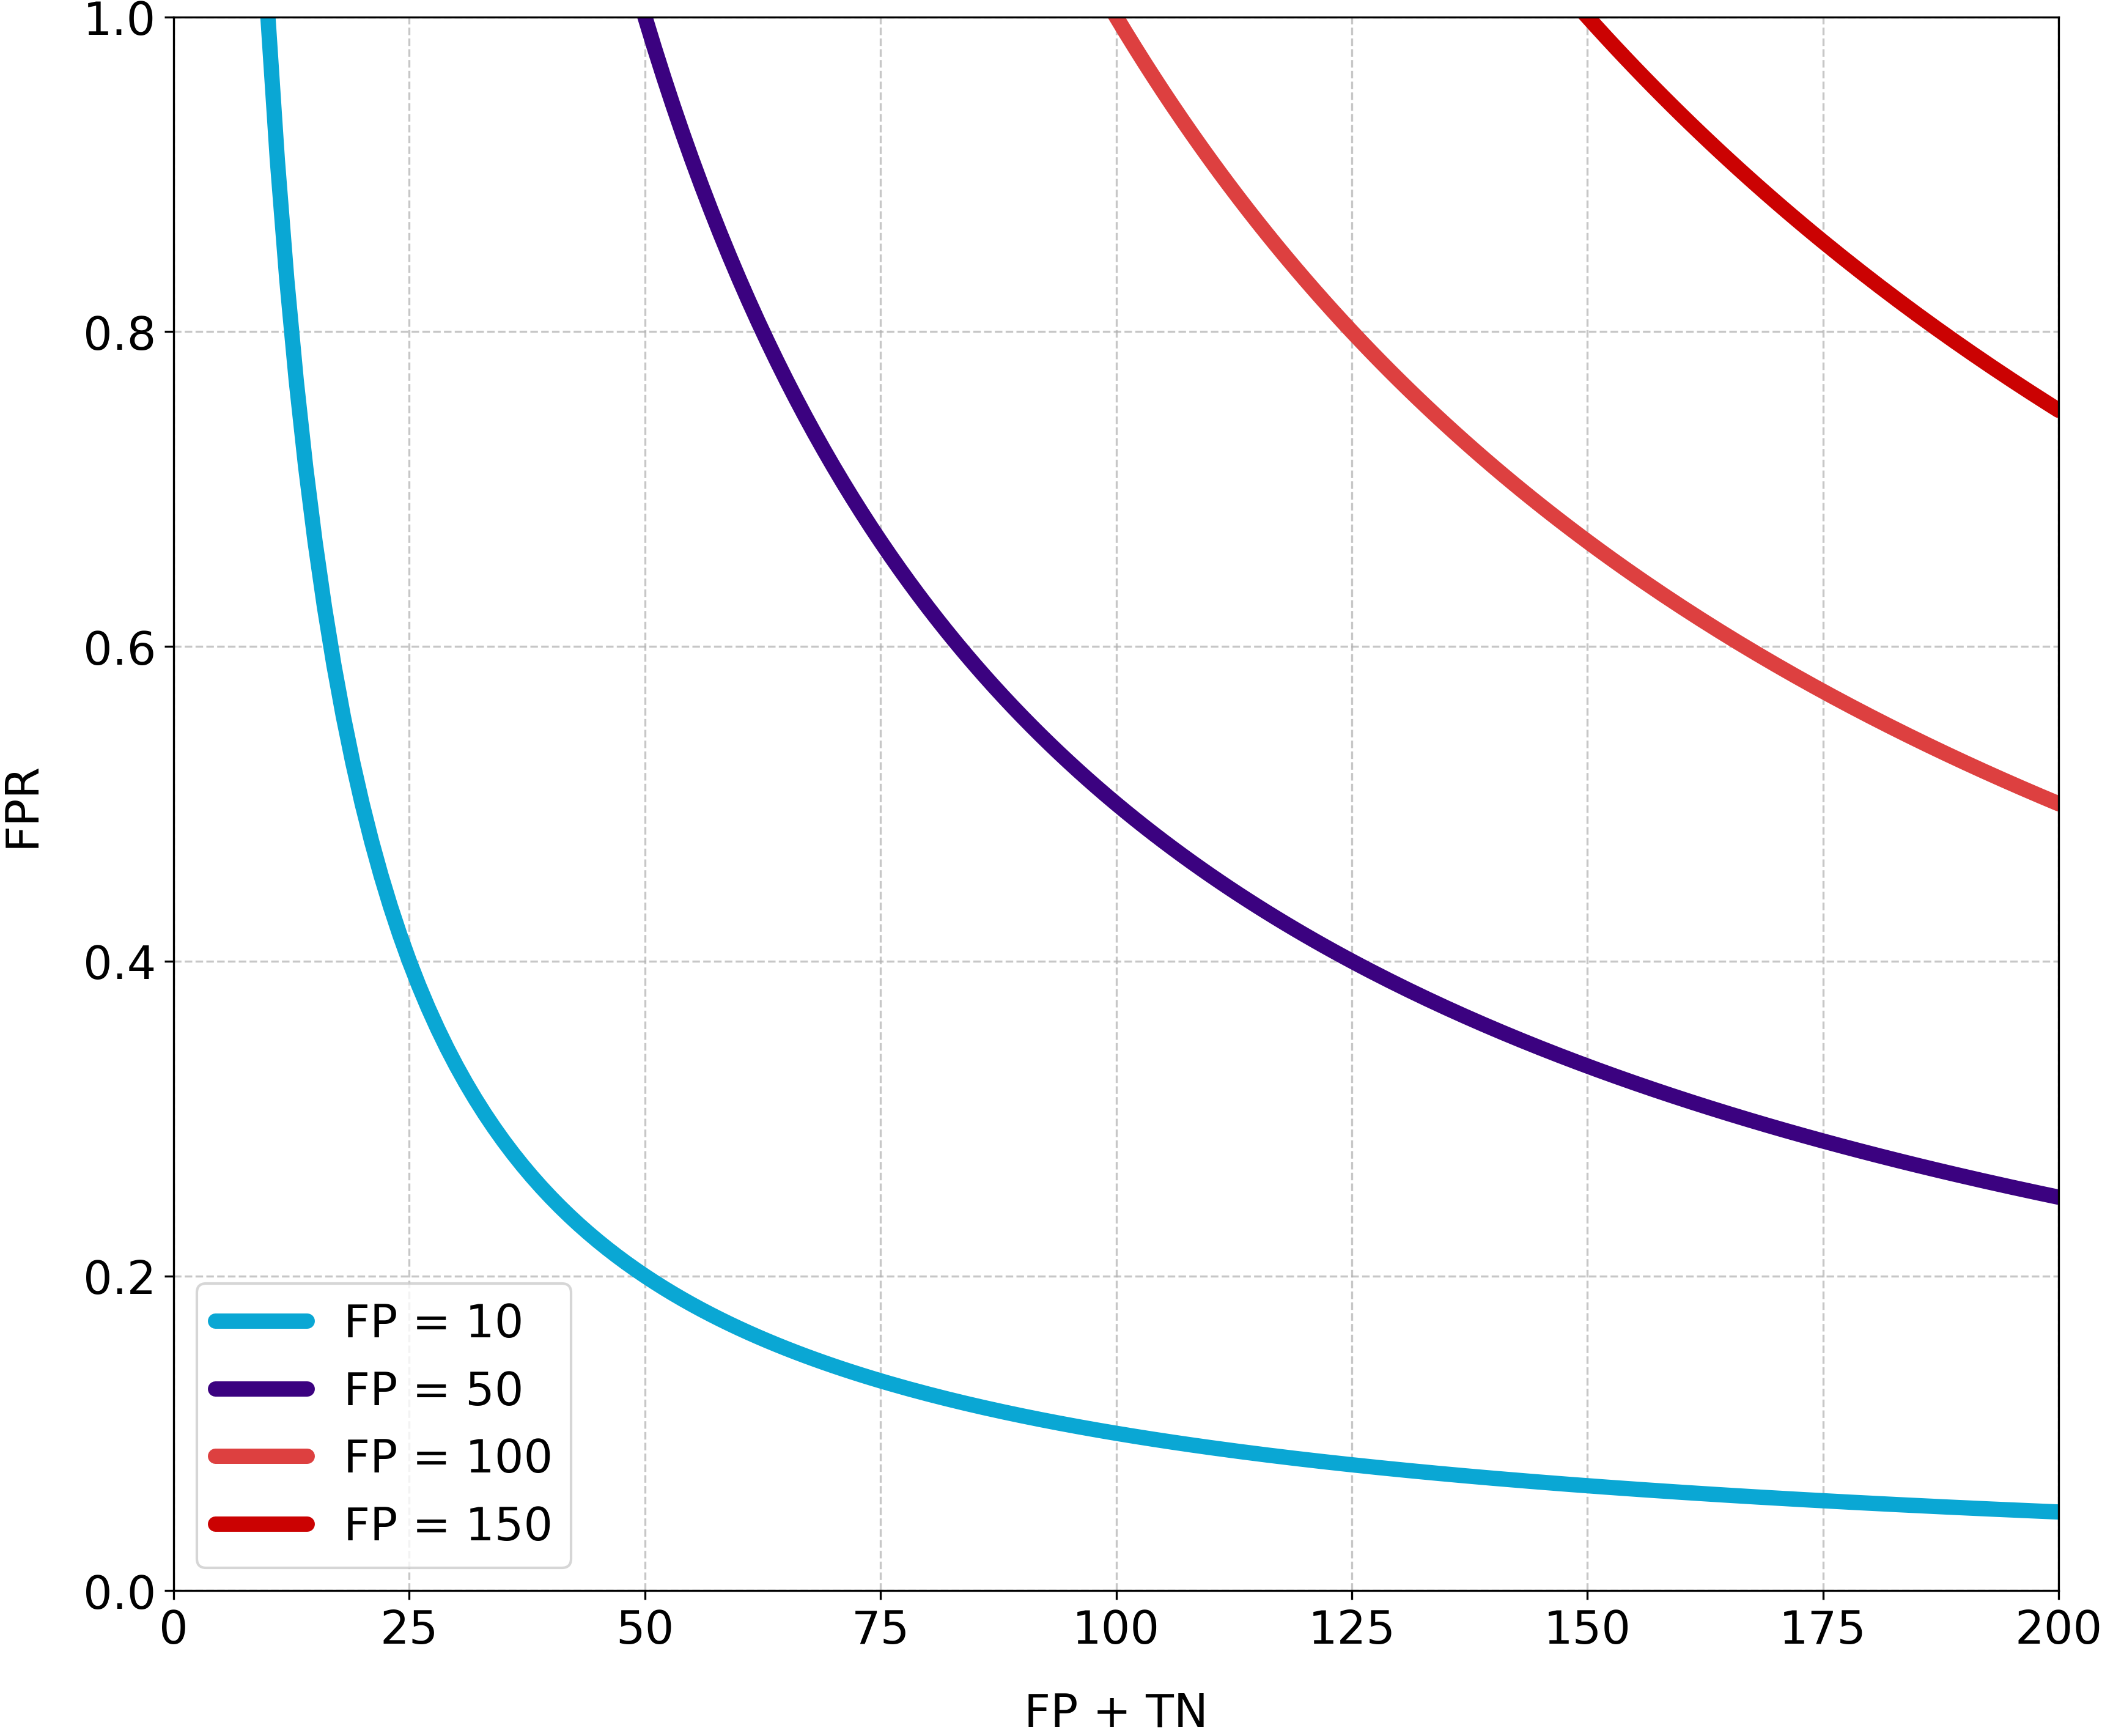
\includegraphics[width=0.5\textwidth]{figures/FPR_2d_line_plot.png} % Your figure goes here
\end{wrapfigure}

% Left text with the image on the right
\textbf{Figure 3.1 False Positive Rate.} 
\textbf{Top:}
3D surface illustrating FPR's non-linear relationship with FP and TN. FPR is lowest (blue) when FP is low. It increases (red) as FP increases.
\textbf{Right:}
Shows how FPR decreases hyperbolically as total negative cases increase for fixed FP values. Lower FP maintains better FPR.


\orangebox{%
Did you know that...}
{
In the context of statistical hypothesis testing, the FPR is also known as the "type I error rate" or the probability of rejecting a true null hypothesis.
}

\textbf{FPR alternatives and related metrics}

Other metrics used alongside or instead of FPR include True Positive Rate (TPR), Precision, F1-Score, Receiver Operating Characteristic (ROC AUC), and Specificity.


% ---------- FNR ----------
\clearpage
\section{FNR}
\subsection{False Negative Rate}
\thispagestyle{classificationstyle}

The False Negative Rate (FNR), also known as the miss rate, measures the proportion of actual positive instances incorrectly classified as negative in binary classification.
\begin{center}
\tikz{
\node[inner sep=2pt, font=\Large] (a) {
{
$\displaystyle
FPR = \frac{{\color{cyan}FP}}{{\color{cyan}FP} + {{\color{nmlpurple}TN}}}
$
}
};
\draw[-latex,cyan, semithick] ($(a.north)+(1.3,0.05)$) to[bend left=15] node[pos=1, right] {False positives} +(1,.5); 
% \draw[-latex,teal!70!green, semithick] ($(a.south)+(2.1,0.1)$) to[bend right=15] node[pos=1, right] {Mean of targets} +(1,-.5); 
\draw[-latex,nmlpurple, semithick] ($(a.south)+(1.5,-0.05)$) to[bend left=15] node[pos=1, left] {True negatives} +(-1,-.5); 
}
\end{center}

FNR ranges from 0 (no false negatives) to 1 (all positive instances misclassified). It represents the probability that a positive instance will be incorrectly identified as negative.

\textbf{When to use FNR?}

Use FNR when the cost of missing positive cases is high (e.g., in medical diagnostics or fraud detection) or when you must balance false negatives and false positives.

\coloredboxes{
\item It directly measures the rate of missed positive cases.
\item It is critical in fields where false negatives have severe consequences.
\item Complements True Positive Rate (TPR) in assessing classifier performance.
}
{
\item It doesn't account for true negatives or false positives.
\item It can be misleading in highly imbalanced datasets.
\item It should be considered alongside other metrics for a comprehensive evaluation.
}


\clearpage
\thispagestyle{customstyle2}


\begin{figure*}[ht!]
    \centering
    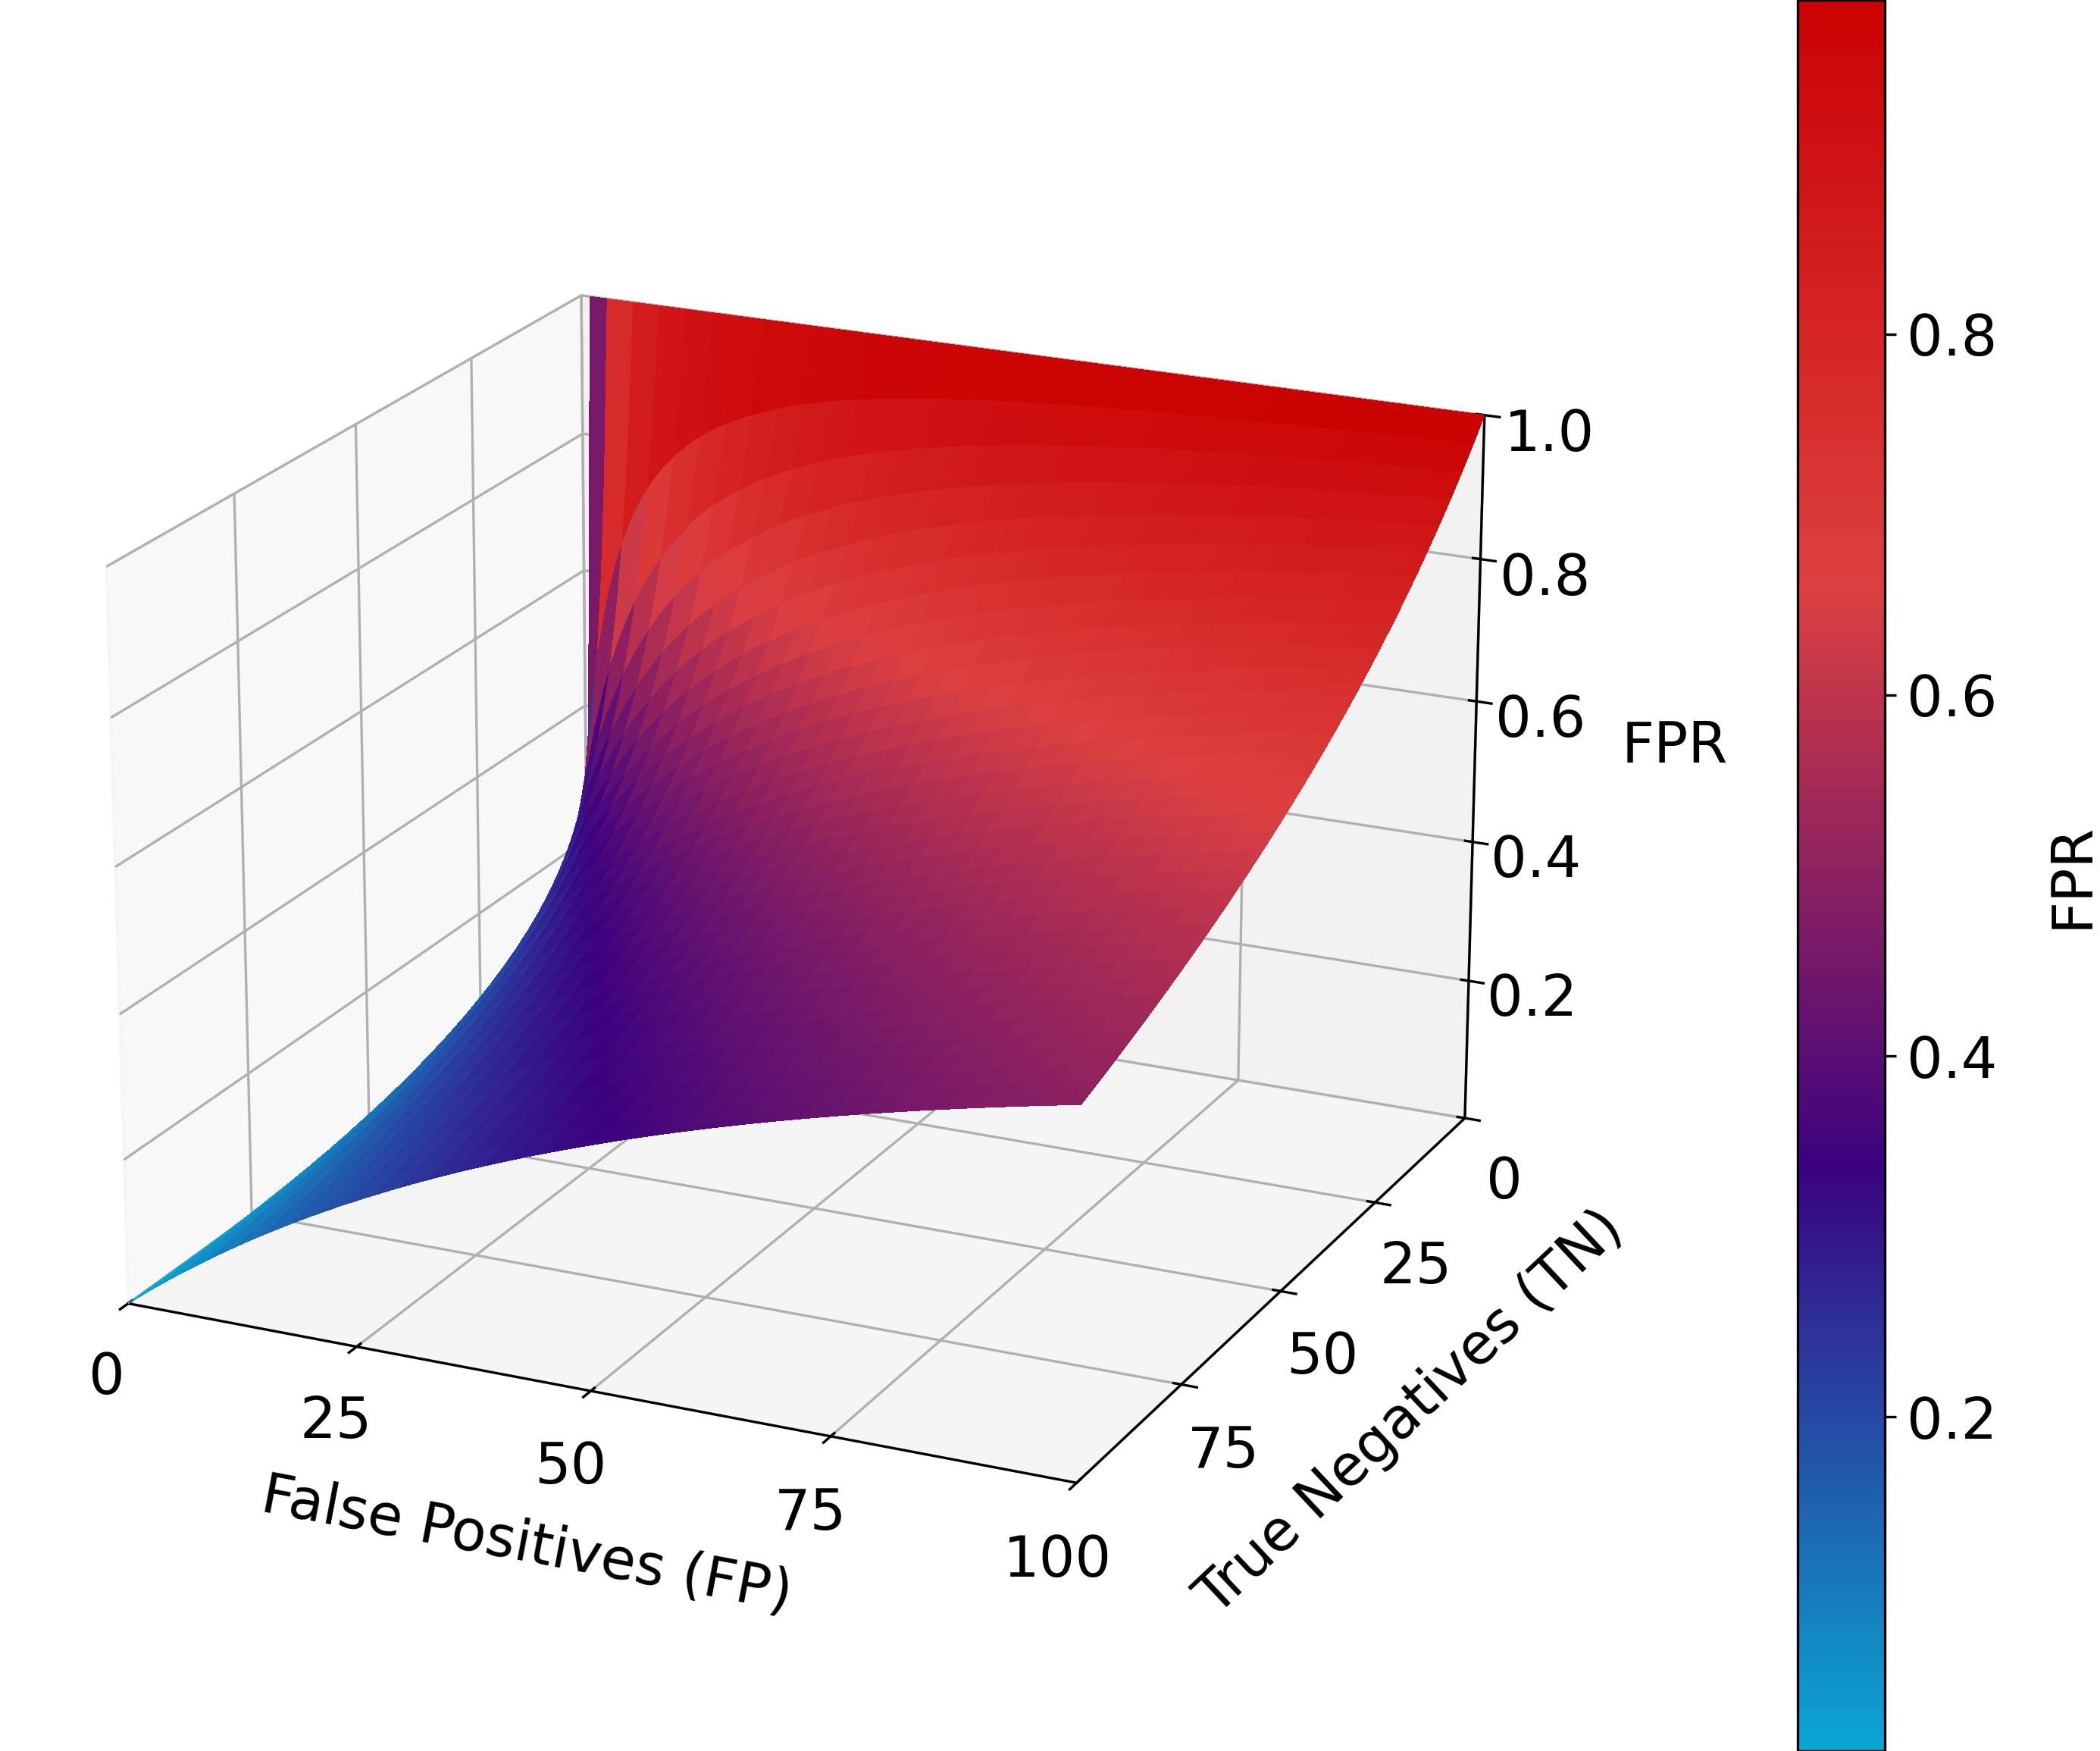
\includegraphics[width=0.7\textwidth]{figures/FPR_3d_surface.png}
    % \caption{Caption}
    \label{fig1}
\end{figure*}

\begin{wrapfigure}{r}{0.55\textwidth}
    \centering
    \vspace{-20pt} % Adjust vertical alignment if needed
    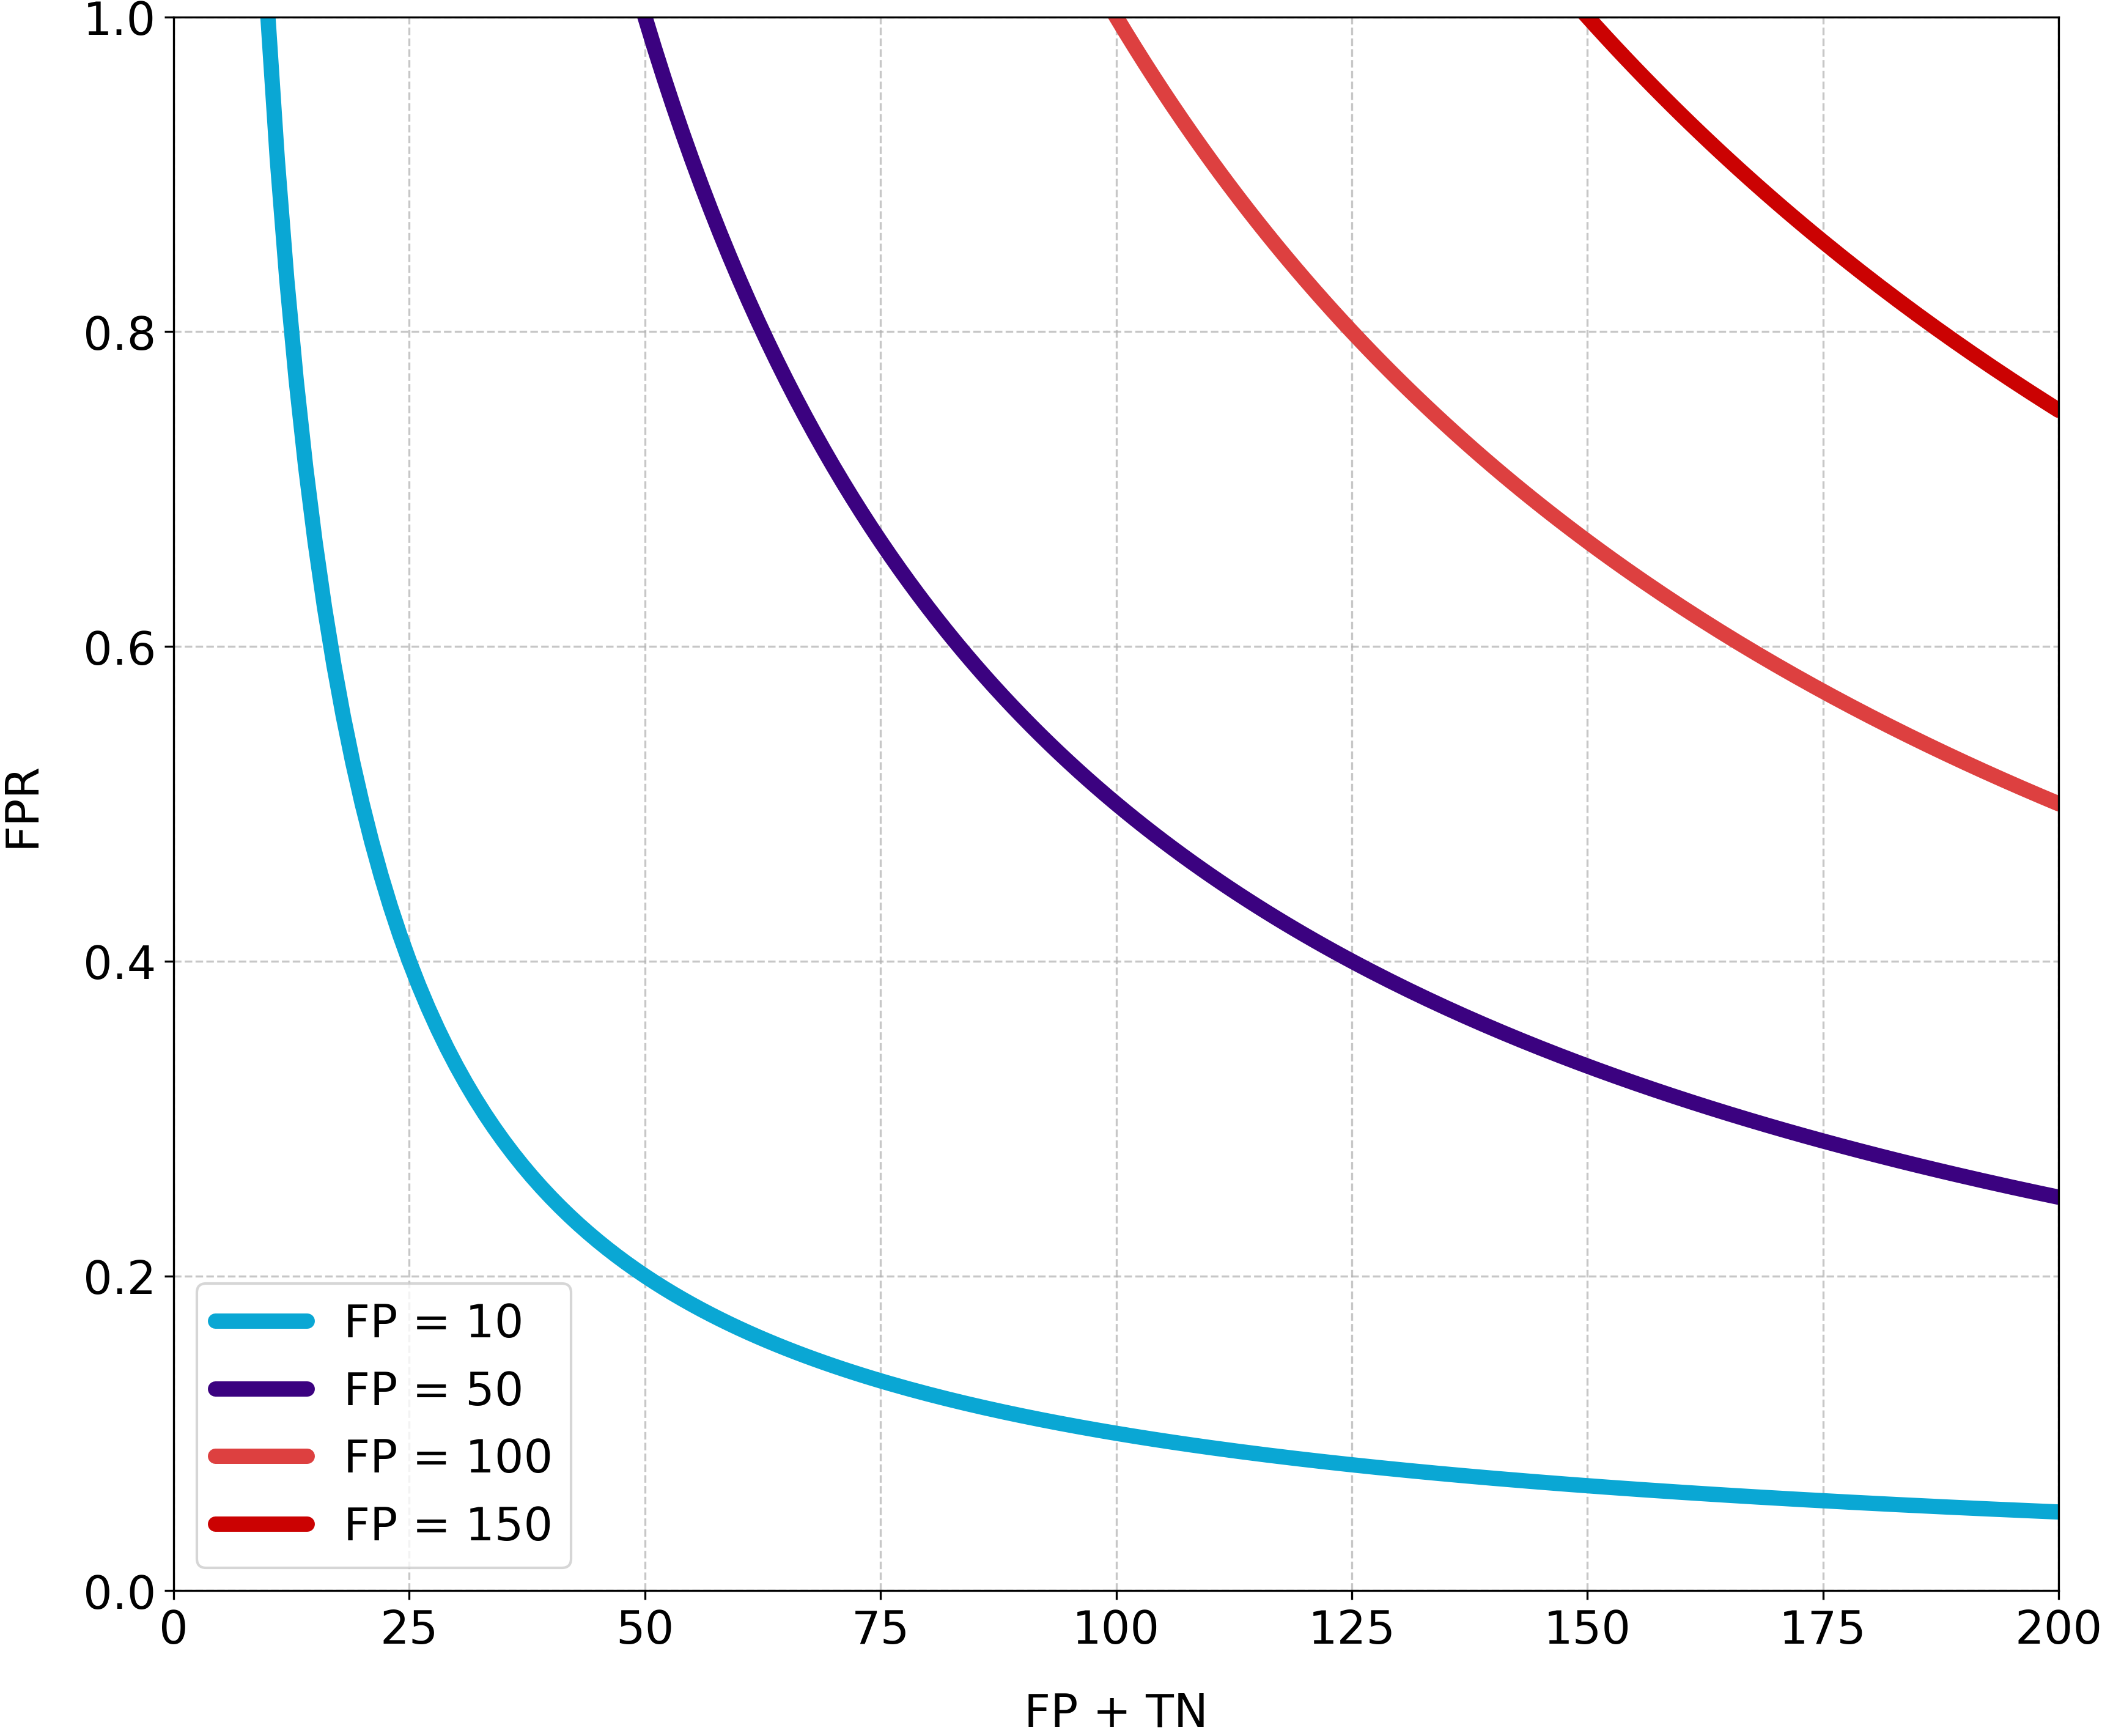
\includegraphics[width=0.5\textwidth]{figures/FPR_2d_line_plot.png} % Your figure goes here
\end{wrapfigure}

% Left text with the image on the right
\textbf{Figure 3.1 False Negative Rate.} 
\textbf{Top:}
3D surface illustrating FPR's non-linear relationship with FP and TN. FPR is lowest (blue) when FP is low. It increases (red) as FP increases.
\textbf{Right:}
Shows how FPR decreases hyperbolically as total negative cases increase for fixed FP values. Lower FP maintains better FPR.


\orangebox{%
Did you know that...}
{
    In hypothesis testing, reducing the False Negative Rate ($\beta$) increases the power of the test ($1 - \beta$), but often at the cost of increasing the False Positive Rate ($\alpha$).
    This demonstrates the inherent trade-off between Type I and Type II errors in statistical testing.
}

\textbf{FPR alternatives and related metrics}

Other metrics used alongside or instead True Positive Rate (TPR/Recall/Sensitivity), Specificity, Precision, F1-Score, and ROC curve.

% ---------- FNR ----------
\clearpage
\thispagestyle{customstyle}
\section{FNR}
\subsection{False Negative Rate}

% ---------- TPR ----------
\clearpage
\thispagestyle{customstyle}
\section{TPR}
\subsection{True Positive Rate (Recall/Sensitivity)}

% ---------- TNR ----------
\clearpage
\thispagestyle{customstyle}
\section{TNR}
\subsection{True Negative Rate (Specificity)}

% ---------- Accuracy ----------
\clearpage
\thispagestyle{customstyle}
\section{Accuracy}
\subsection{Accuracy}

% ---------- Balanced Accuracy ----------
\clearpage
\thispagestyle{customstyle}
\section{Balanced Accuracy}
\subsection{Balanced Accuracy}

% ---------- Precision ----------
\clearpage
\thispagestyle{customstyle}
\section{Precision}
\subsection{Precision}

% ---------- F1-score ----------
\clearpage
\thispagestyle{customstyle}
\section{F1-score}
\subsection{F1-score}

% ---------- F-beta ----------
\clearpage
\thispagestyle{customstyle}
\section{F-beta}
\subsection{F-beta}

% ---------- F-beta ----------
\clearpage
\thispagestyle{customstyle}
\section{F-beta}
\subsection{F-beta}

% ---------- ROC AUC ----------
\clearpage
\thispagestyle{customstyle}
\section{ROC AUC}
\subsection{Area Under the Receiver Operating Characteristic Curve}

% ---------- PR AUC ----------
\clearpage
\thispagestyle{customstyle}
\section{PR AUC}
\subsection{Area Under the Precision-Recall Curve}

% ---------- Brier Score Loss ----------
\clearpage
\thispagestyle{customstyle}
\section{Brier Score Loss}
\subsection{Brier Score Loss}

% ---------- Log Loss ----------
\clearpage
\thispagestyle{customstyle}
\section{Log Loss}
\subsection{Log Loss}

% ---------- Jaccard Score ----------
\clearpage
\thispagestyle{customstyle}
\section{Jaccard Score}
\subsection{Jaccard Score}

% ---------- D2 Log Loss Score ----------
\clearpage
\thispagestyle{customstyle}
\section{D2 Log Loss Score}
\subsection{D2 Log Loss Score}

% ---------- P4-metric ----------
\clearpage
\thispagestyle{customstyle}
\section{P4-metric}
\subsection{P4-metric}

% ---------- Cohen's Kappa ----------
\clearpage
\thispagestyle{customstyle}
\section{Cohen's Kappa}
\subsection{Cohen's Kappa}

% ---------- Phi Coefficient ----------
\clearpage
\thispagestyle{customstyle}
\section{Phi Coefficient}
\subsection{Phi Coefficient}

% ---------- MCC ----------
\clearpage
\thispagestyle{customstyle}
\section{MCC}
\subsection{Matthew's Correlation Coefficient}